\subsection{题目描述}
\noindent Use the file called \texttt{sunspots.txt}, which contains the observed number of sunspots on the Sun for each month since January 1749. Write a program to calculate the Fourier transform of the sunspot data and then make a graph of the magnitude squared \( |c_k|^2 \) of the Fourier coefficients as a function of \( k \)—also called the power spectrum of the sunspot signal. You should see that there is a noticeable peak in the power spectrum at a nonzero value of \( k \). Find the approximate value of \( k \) to which the peak corresponds. What is the period of the sine wave with this value of \( k \)?

\noindent \textit{Special note:} You may use any built-in functions for the Fourier transform.


\subsection{程序描述}
使用\texttt{scipy}库的\texttt{detrend}函数去除线性趋势,也进行了使用Hanning窗平滑过渡原信号
\[
w(n) = 0.5 \left( 1 - \cos\left( \frac{2\pi n}{N-1} \right) \right)
\]
的效果对比,该操作有效避免边缘频率泄露,最后使用\texttt{np.fft}进行快速傅里叶变换,得到频谱图并使用\texttt{np.fft.ifft}进行信号重构的对比。最终峰值频率对应周期为$130.6 m\approx10.9 a$,与太阳黑子爆发周期实验观测值相符。

源代码在\texttt{src/analysis.py}中,请在该目录下运行\ccmd{python -u analysis.py}即可得到结果,需要安装\texttt{numpy}与\texttt{scipy}库辅助运算,\texttt{matplotlib}库绘图,其他平台运行可能需要调整字体管理代码。
\subsection{结果示例}
\begin{figure}[H]
    \centering
    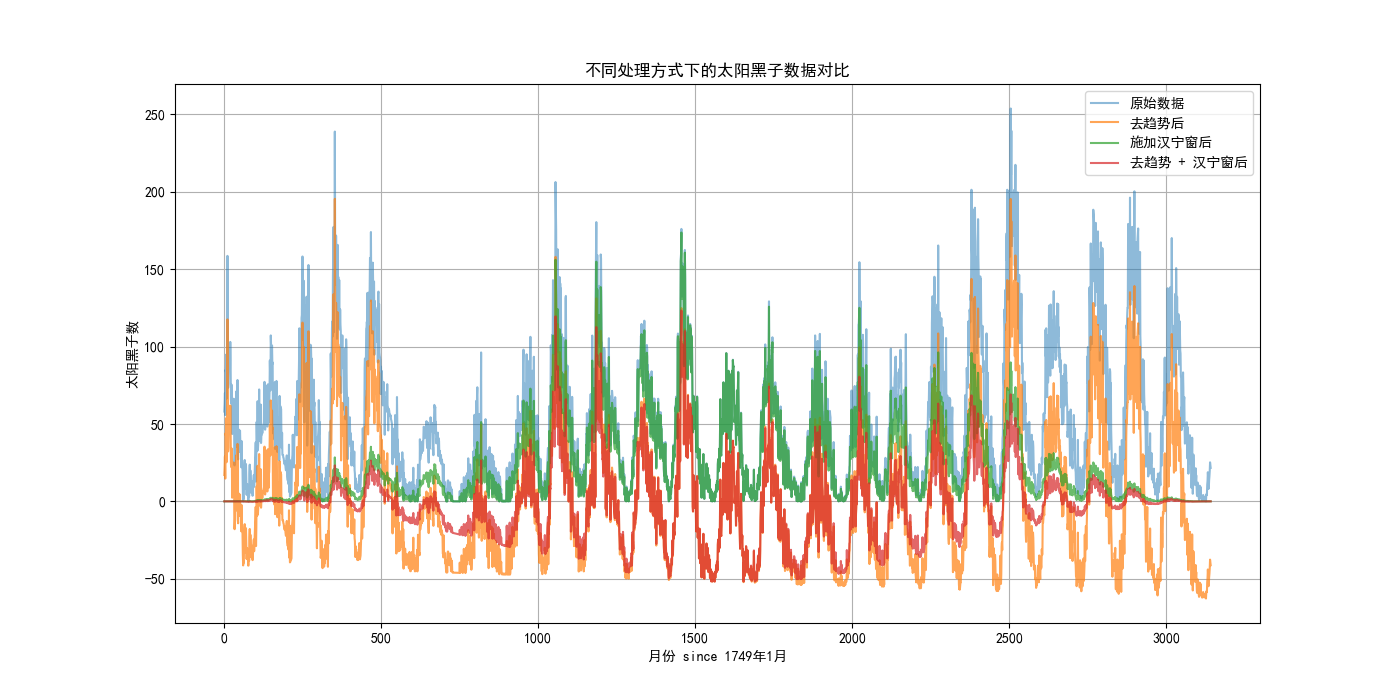
\includegraphics[width=1.0\textwidth]{Problem_2/figs/comparison.png}
    \caption{不同方式处理的数据对比}
\end{figure}

\begin{figure}[H]
    \centering
    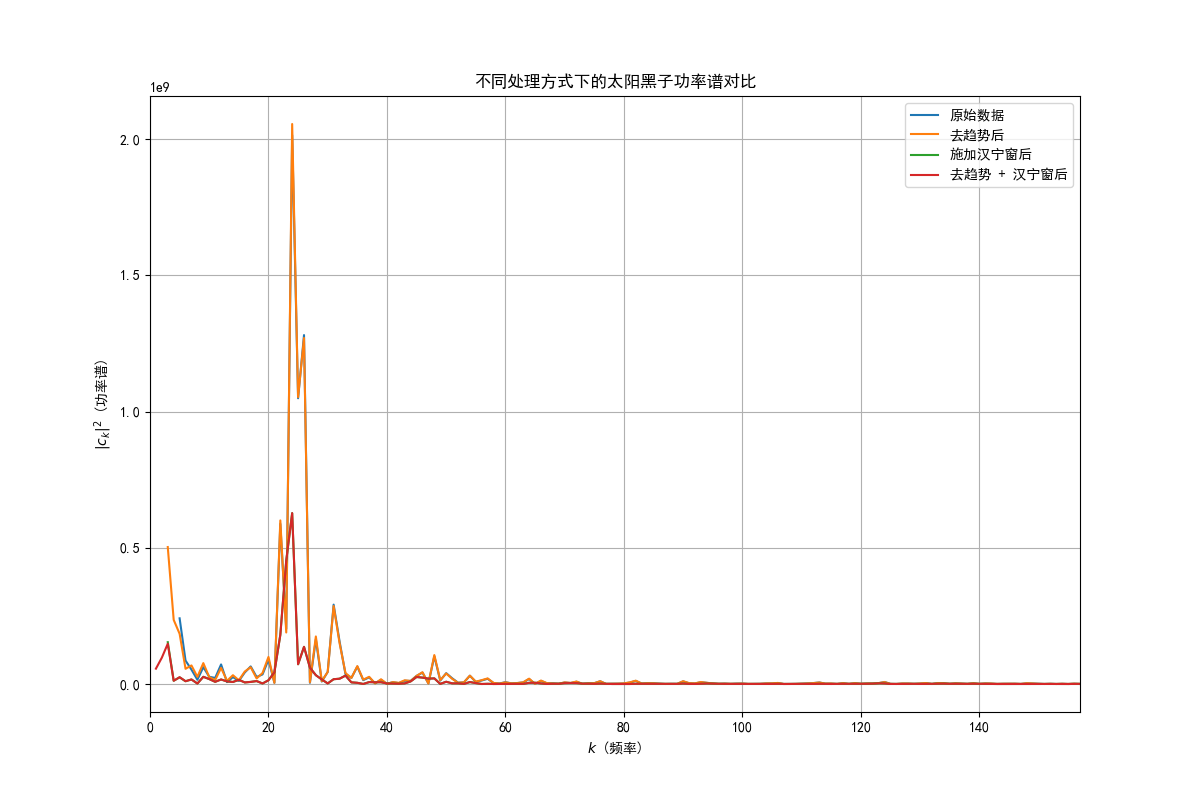
\includegraphics[width=0.8\textwidth]{Problem_2/figs/spectrum.png}
    \caption{去趋势+汉宁窗处理后的功率谱}
\end{figure}

\begin{figure}[H]
    \centering
    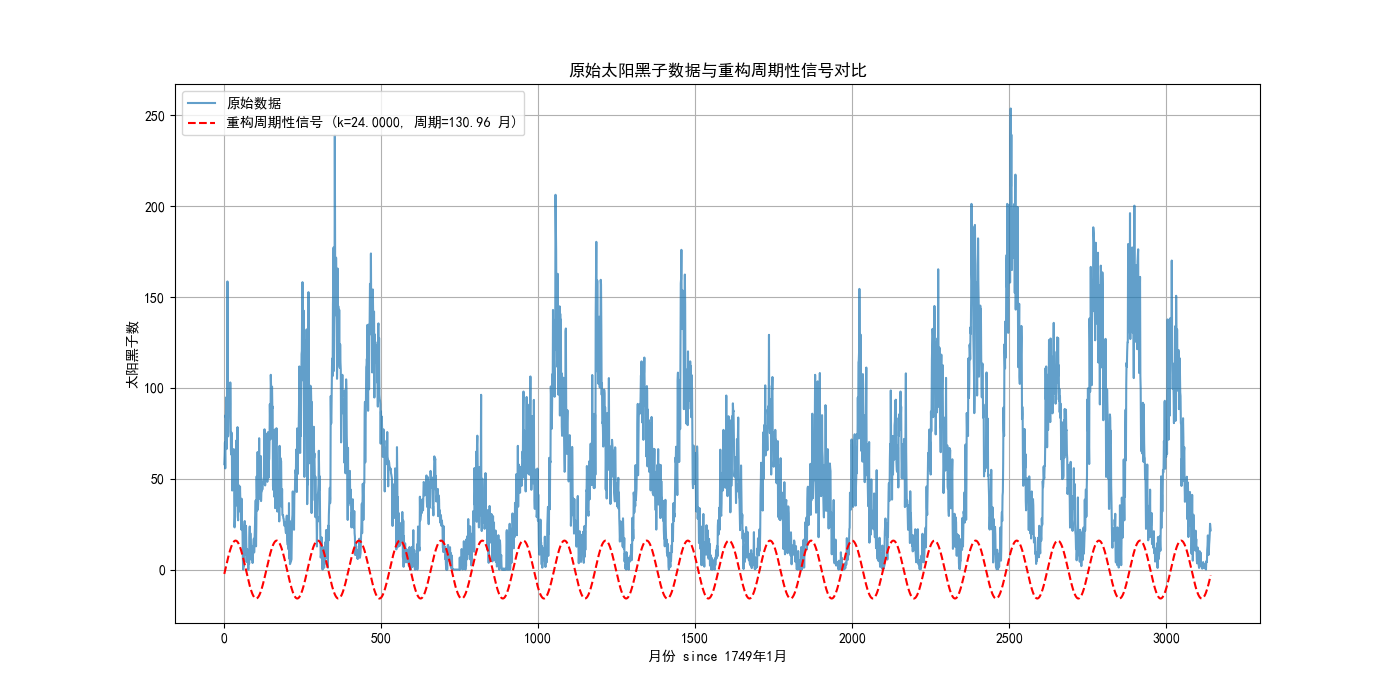
\includegraphics[width=0.8\textwidth]{Problem_2/figs/reconst.png}
    \caption{使用峰值频率重构与原信号对比}
\end{figure}
